\documentclass[border=4pt]{standalone}
\usepackage{amsmath}
\usepackage{amssymb}
\usepackage{tikz}
\usetikzlibrary{positioning,arrows.meta,fit,calc,shadows}
\begin{document}
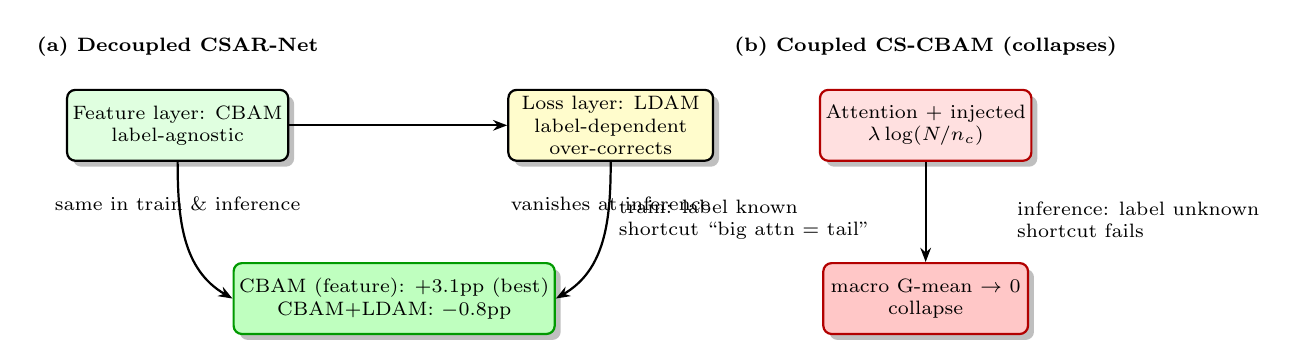
\begin{tikzpicture}[
			mod/.style={rectangle,draw,thick,rounded corners=3pt,minimum height=0.9cm,minimum width=2.6cm,font=\scriptsize,align=center,inner sep=2pt,drop shadow},
			lab/.style={font=\scriptsize,align=left},
			arr/.style={-{Stealth[length=1.8mm]},thick},
		]
			% ---- (a) decoupled ----
			\node[lab] at (0,0) {\textbf{(a) Decoupled CSAR-Net}};
			\node[mod,fill=green!12] (f) at (0,-1.0) {Feature layer: CBAM\\label-agnostic};
			\node[mod,fill=yellow!20] (l) at (5.5,-1.0) {Loss layer: LDAM\\label-dependent\\over-corrects};
			\node[lab] at (0,-2.0) {same in train \& inference};
			\node[lab] at (5.5,-2.0) {vanishes at inference};
			\node[mod,fill=green!25,draw=green!60!black] (ok) at (2.75,-3.2) {CBAM (feature): $+$3.1pp (best)\\CBAM$+$LDAM: $-$0.8pp};
			\draw[arr] (f)--(l);
			\draw[arr] (f.south) to[out=-90,in=150] (ok.west);
			\draw[arr] (l.south) to[out=-90,in=30] (ok.east);

			% ---- (b) coupled ----
			\node[lab] at (9.5,0) {\textbf{(b) Coupled CS-CBAM (collapses)}};
			\node[mod,fill=red!12,draw=red!70!black] (cf) at (9.5,-1.0) {Attention $+$ injected\\$\lambda\log(N/n_c)$};
			\node[lab] at (7.2,-2.2) {train: label known\\shortcut ``big attn $=$ tail''};
			\node[lab] at (12.2,-2.2) {inference: label unknown\\shortcut fails};
			\node[mod,fill=red!22,draw=red!70!black] (bad) at (9.5,-3.2) {macro G-mean $\to$ 0\\collapse};
			\draw[arr] (cf.south) to[out=-90,in=90] (bad.north);
		\end{tikzpicture}
\end{document}
